\documentclass[11]{beamer}
\usepackage{hyperref}
\usepackage{graphicx} % Allows including images
\usepackage{booktabs} % Allows the use of \toprule, \midrule and \bottomrule in tables
\usepackage{pgfgantt}

% Definições do tema
\usetheme{copenhagen} % Pode ajustar para outro tema se necessário
\usecolortheme{default}
\setbeamertemplate{navigation symbols}{} % Remove os símbolos de navegação

%Information to be included in the title page:
\title{Ferramenta para Geração de Horários de Cursos com Restrições}
\subtitle{Apresentação do Relatório de Desenvolvimento do Trabalho}

\author[Ricardo Ramos]{Ricardo Alexandre Alves Ramos\\
                    \vspace{1em}\footnotesize
                    Orientadores:
                    Prof. Doutor Nuno Miguel da Costa de Sousa Leite\\
                    \hspace{-.6cm} Prof. Doutor Artur Jorge Ferreira}

\institute[ISEL]{Instituto Superior de Engenharia de Lisboa}

%\date{Março 01, 2025}
\date{\today}

\institute{
    Instituto Superior de Engenharia de Lisboa \\ 
    Departamento de Engenharia Eletrónica e de Telecomunicações e Computadores \\ 
    Mestrado em Engenharia Informática e de Computadores
}

\begin{document}
    %----------------------------------------------------------------------------------------
    %    PRESENTATION SLIDES
    %----------------------------------------------------------------------------------------

    % Slide de título
    \frame{\titlepage}

    \begin{frame}{Índice}
        % Throughout your presentation, if you choose to use \section{} and \subsection{} commands, these will automatically be printed on this slide as an overview of your presentation
        \tableofcontents
    \end{frame}

    %------------------------------------------------
    \section{Introdução}
    %------------------------------------------------

    \begin{frame}{Problemas de Agendamento}
        
    \end{frame}

    %------------------------------------------------
    \section{Estado da Arte}
    %------------------------------------------------

    \subsection{Algoritmos tipicamente utilizados}

    \begin{frame}{Algoritmos tipicamente utilizados}
        \begin{itemize}
            \item Procura Tabu
            \item Têmpera Simulada
        \end{itemize}
    \end{frame}

    %------------------------------------------------
    \section{Trabalho Realizado}
    %------------------------------------------------

    \begin{frame}
        \begin{itemize}
            \item 
            \item 
        \end{itemize}
    \end{frame}

    %------------------------------------------------
    \section{Trabalho Futuro}
    %------------------------------------------------

    \subsection{Diagrama de Gantt}

    \begin{frame}{Diagrama de Gantt}
        \begin{figure}
            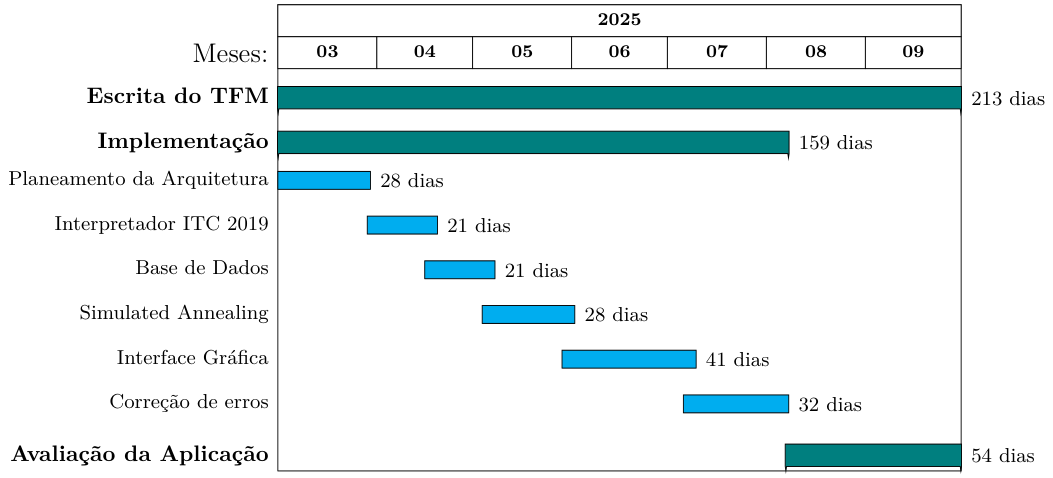
\includegraphics[width=\linewidth]{img/Diagrama-Gantt.png}
            \caption{Diagrama de Gantt}
        \end{figure}
    \end{frame}

    %----------------------------------------------------------------------------------------

\end{document}